\section{Introduction}
\label{section_ztf_intro}
Zwicky Transient Facility (\href{https://www.ztf.caltech.edu/}{ZTF}) is a time-domain survey of the northern sky
that had first light at Palomar Observatory in 2017.  It is run by CalTech.
My advisor Pavlos suggested it as a data source for this project.
The ZTF dataset has two major advantages for searching for asteroids:
\begin{itemize}
\item ZTF gives a wide and fast survey of the key, covering over 3750 square degrees an hours to a depth of 20.5 mag
\item A machine learning pipeline has been developed to classify a subset of ZTF detections that are classified as probable asteroids
\end{itemize}
The data set I analyze here consists of all ZTF detections that were classified as asteroids.
Data on each detection include:
\begin{itemize}
\item \textbf{ObjectID} an identifier of the likely ojbect associated with this detection; multiple detections often share the same ObjectID
\item \textbf{CandidateID} a unique integer identifier of each detection
\item \textbf{MJD} The time of the detection as an MJD
\item \textbf{RA} The right ascension of the detection
\item \textbf{Dec} The declination of the detection
\item \textbf{mag} The apparent magnitude of the detection
\end{itemize}
Available data also includes a number of additional fields that were not used in the analysis.

\href{https://github.com/alercebroker}{ALeRCE} (Automatic Learning for the Rapid Classification of Events) is an astronomical data broker.
ALeRCE provides a convenient API to access the ZTF asteroid data, which can be installed with \tty{pip}.
I used ALeRCE on this project to download the ZTF asteroid data set.

\section{Exploratory Data Analysis of ZTF Asteroid Data}
\label{section_ztf_eda}
Before plowing into the search for new asteroids, I conducted an exploratory data analysis (EDA) of the ZTF asteroid dataset.
This can be followed interactively in the Jupyter notebook \tty{05\_ztf\_data.ipynb}.
I took a download of the data running through 26-Feb-2020.
The first detection is on 01-Jun2018.
The dataset contains 5.69 total detections.  
The volume of detections increases very significantly beginning in July 2019; 
for practical purposes the dataset consists of 8 months of detections spanning July 2019 through February 2020.

\begin{figure}[hbt!]
\begin{center}
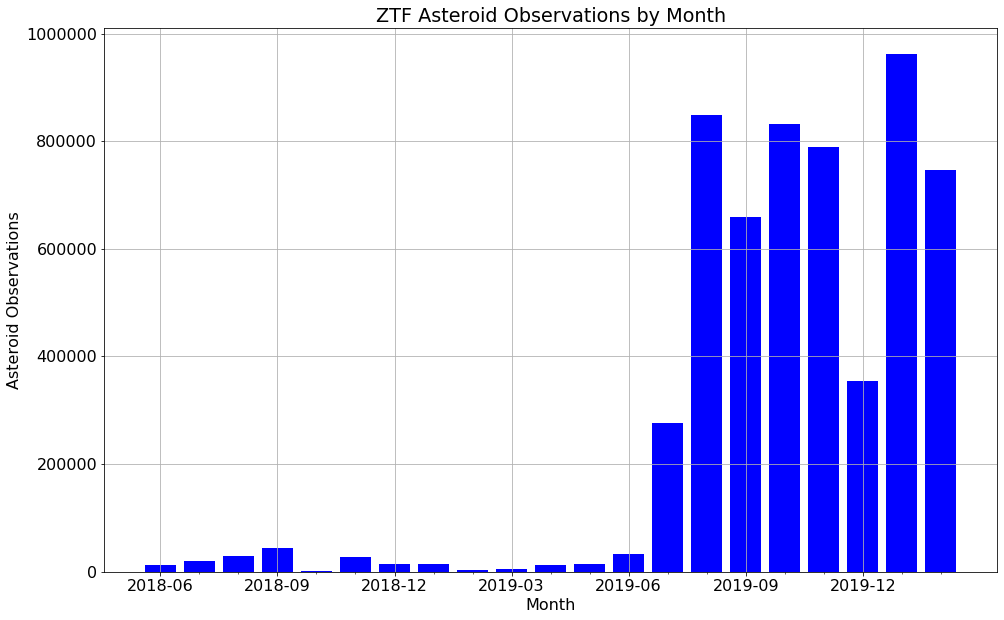
\includegraphics[width=0.85\textwidth]{../figs/ztf/ztf_ast_per_month.png}
\caption{ZTF Asteroid Detections per month}
\end{center}
\end{figure}

\begin{figure}[hbt!]
\begin{center}
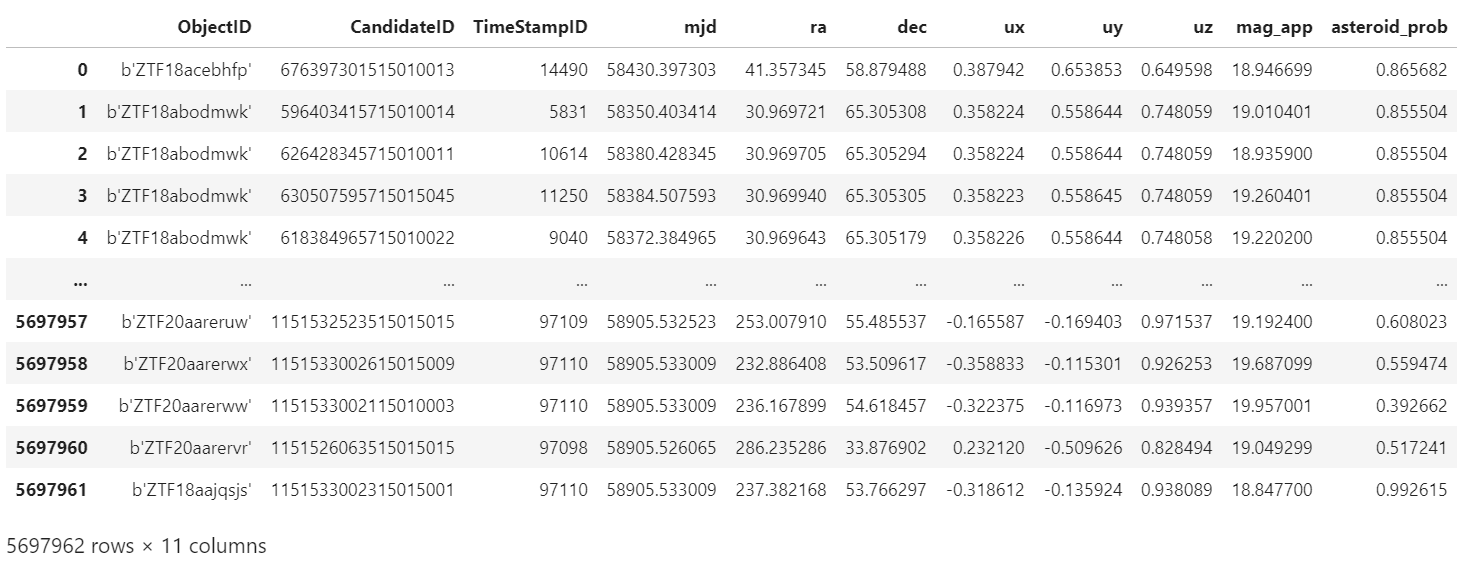
\includegraphics[width=1.0\textwidth]{../figs/ztf/ztf_dataframe.png}
\caption{Preview of Pandas DataFrame of ZTF Detections}
\end{center}
\end{figure}

The fields \tty{mjd}, \tty{ra}, \tty{dec}, and \tty{mag\_app} are part of the original dataset.
I have populated the columns \tty{ux}, \tty{uy} and \tty{uz} by running \tty{radec2dir} on the quoted RA/Dec from ZTF.

Here is a chart showing the distribution of apparent magnitudes in the ZTF detections.
It's shown on a log scale because there are so many more detections around the peak 19.5
than at the brightest (10) and and dimmest (22) magnitudes. 
\begin{figure}[hbt!]
\begin{center}
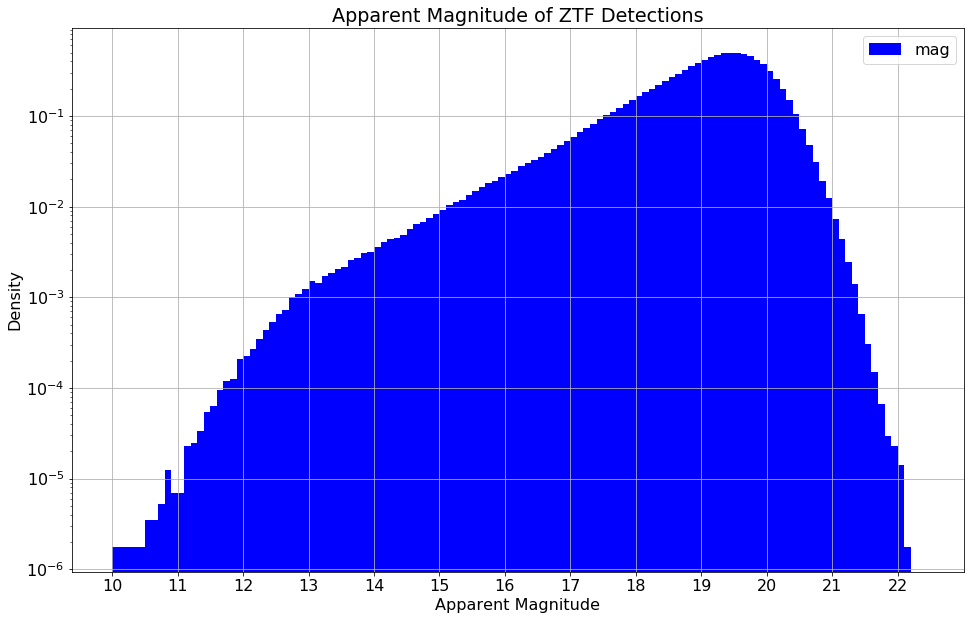
\includegraphics[width=0.85\textwidth]{../figs/ztf/apparent_mag.png}
\caption{Apparent Magnitude of ZTF asteroid detections.}
\end{center}
\end{figure}
\clearpage

\section{The Angular Distance Bewteen two Directions $\vec{u}_1$ and $\vec{u}_2$}
\label{section_ztf_angle_diff}
A recurring task in this thesis to compute the angular distance bewteen two directions on the unit sphere.
If $\uvec_1$ and $\uvec_2$ are on the unit sphere, we can compute their Cartesian distance $s$ in the usual way,
$$ s = \norm{\uvec_2 - \uvec_1}$$
$s$ will be in the interval $[0, 2]$.
We would also like to know the angular distance $\theta$ of the shortest path 
on the surface of the sphere (geodesic) connecting these two points.
On Earth, this would be analogous to the length of the great circle route by airplane between two cities.
Here is a simple picture demonstrating the derivation of the formula relating $s$ and $\theta$.
\begin{figure}[hbt!]
\begin{center}
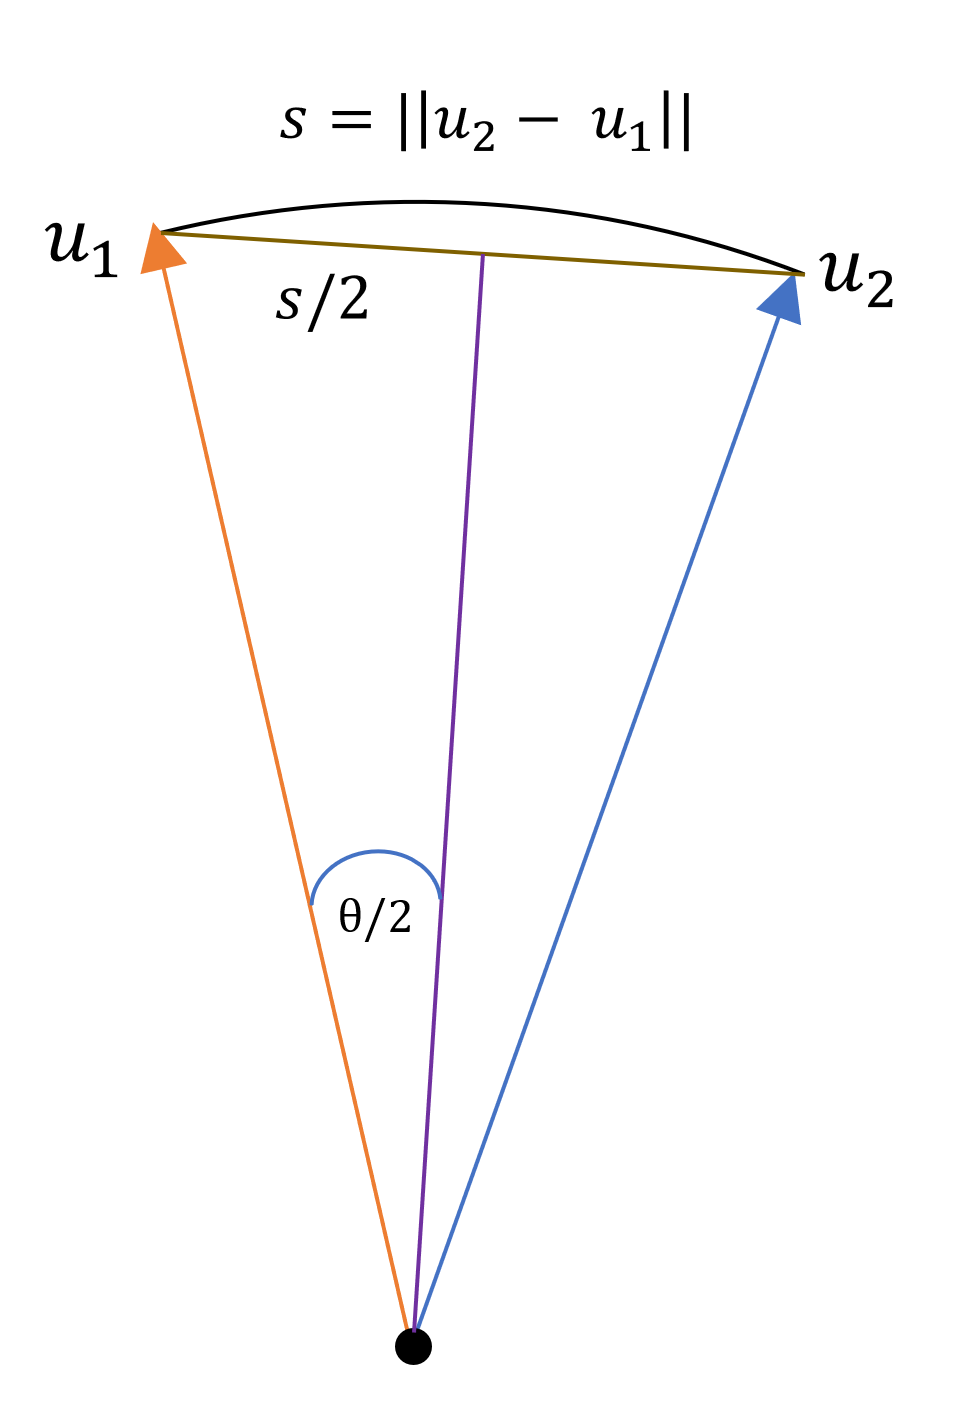
\includegraphics[width=0.3\textwidth]{../figs/misc/angular_distance.png}
\caption{The angular distance between two directions on the unit sphere.}
\end{center}
\end{figure}
The two directions are shown as arrows pointing up.
The distance between them $s$ is bisected by a line segment from the center of the sphere.
This forms a right triangle with hypotenuse $1$ and side length $s/2$ opposite angle $\theta/2$.
We thus obtain the formulas
\begin{align*}
\sin (\theta / 2) &= s / 2 \\ 
\theta &= 2 \arcsin (s / 2) \\
s &= 2 \sin \theta (\theta / 2)
\end{align*}
This function is implemented in \tty{astro\_utils} as \tty{deg2dist} and \tty{dist2deg} to convert between degrees and Cartesian distance in either direction.

\section{Finding the Nearest Asteroid to Each ZTF Detection}
\label{section_ztf_nearest_ast}
We now have in principle all the tools required to find which asteroid was closest in angular distance to each ZTF observation.
To recap the key steps, each ZTF observation is converted from a RA/Dec to a direction in the BME.
The position of Earth and each of the 733,489 catalogued asteroids are integrated as of the objervation time, and the direction bewteen them is calculated.
There are a few problems with the brute force approach implicitly suggested above.
We have 5.7E6 detections and 7.3E5 catalogued asteroids for a total of 4.16E12 (4.16 billion) interactions.
Even if we work in single precision with 4 bytes per float, we need 12 bytes for a 3D direction difference translating to about 50 GB to load the matrix in memory.
The bigger problem is that a brute force integration of all the asteroids at the MJDs of the all 5.7 million observations would be brutally slow.

Fortunately there are a few simple tricks we can use that together make this problem tractable.
The ZTF detections come from a series of images taken through the same telescope, so they come in blocks made at the same time.
The 5.7 million rows share ``only'' 97,111 distinct MJDs.
We also don't need to re-integrate the asteroid orbits.
We've already done a high precision numerical integration at a 1 day frequency and saved the results into \tty{numpy} arrays in blocks of 1,000 asteroids at a time.
Our entire data span only 635 days.  
Loading one block of 1,000 asteroids therefore has only 3.81 million numbers (635 days x 1,000 asteroids x 6 numbers per integration point).

The code to load the basic ZTF data from ALeRCE is included in the module \tty{ztf\_data.py}.
The main function used by consumers is \tty{load\_ztf\_det\_all}, which loads a cached copy of all the available detections from the local disk.
The module \tty{ztf\_nearest\_ast.py} contains a Python program that peforms the calculation described above.
The block size is a parameter that can be controlled from the commandline; I ended up leaving it at 1,000.
Checking back from my handwritten notes when I ran the job, it took approximately 25 hours to complete on a powerful server with 40 Intel CPU cores.
The job ended up being memory bound, maxxing out all 256 GB of available RAM on the server.
The initial job described above writes only computes the nearest asteroid in a block of 1,000 asteroids.
A second reduction operation is then carried out to find the nearest asteroid overall.
To limit memory usage, this was done in two steps.
First, I took 16 chunks of 1,000 at a time to find the nearest asteroid in a block of 16,000 to each detection.
Then I combined all the blocks of 16,000 (about 46) to generate one file with the nearest asteroid.

The work of splining the asteroid directions is done in the module \tty{asteroid\_dataframe.py}.
It includes functions to load the asteroid data from disk; spline the positions and velocities to the requested dates;
and compute the astrometric directions to these splined positions and velocities.
The module \tty{ztf\_ast} does the work of comparing a block of ZTF observations to a block of splined asteroid directions and finding the nearest one.
Once these calculations have been done once, you don't need to worry about them unless you are adding a new block of ZTF data.
Consumers can load the assembled DataFrame including the nearest asteroid number and distance with 
a single call to \tty{load\_ztf\_nearest\_ast} which is defined in \tty{asteroid\_dataframe}.
For the motivated reader who would like a detailed an interactive review of all these calculations, please see the Jupyter notebook \tty{04\_asteroid\_dataframe.ipynb}.
It includes tests comparing my splined outputs of daily data to Horizons data downloaded at a 3 hour interval.

\begin{figure}[hbt!]
\begin{center}
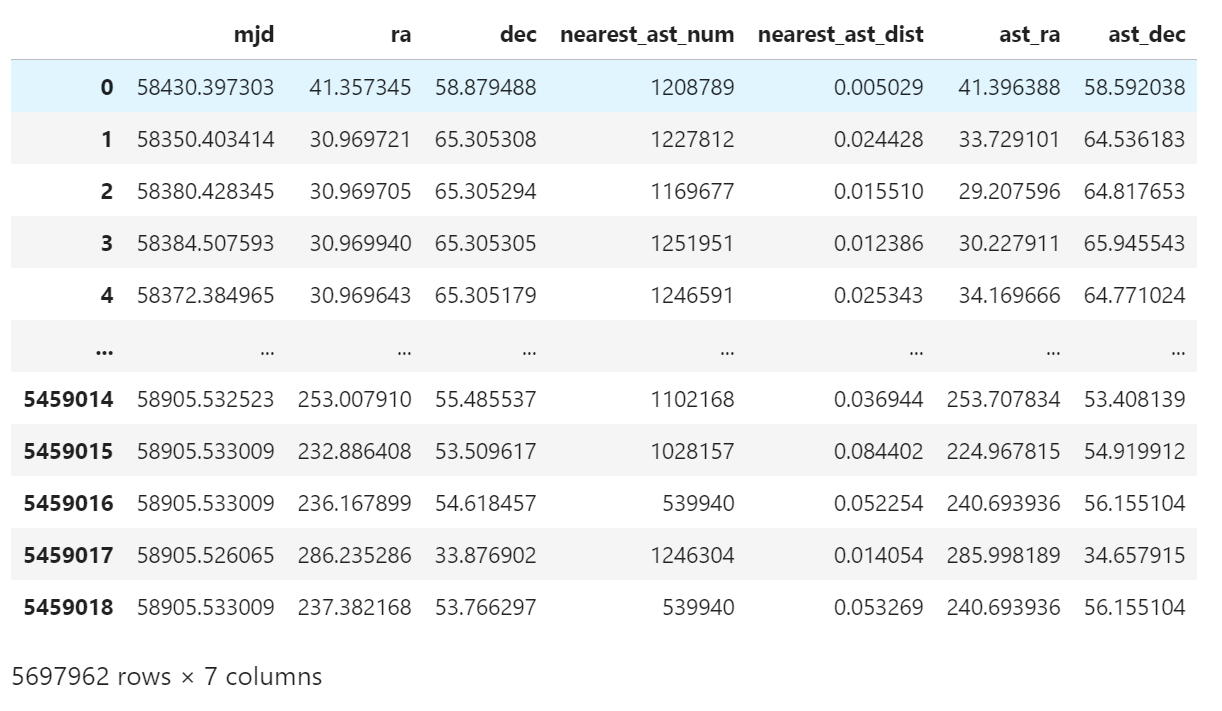
\includegraphics[width=0.9\textwidth]{../figs/ztf/ztf_nearest_ast_dataframe.png}
\caption{Preview of Pandas DataFrame of ZTF Detections Including Nearest Asteroid}
\end{center}
\end{figure}
% \clearpage

One natural question is how the brightness of the nearest asteroid to a detection varies between hits and misses.
The chart below plots two histograms of the absolute magnitude parameter H for the nearest asteroid to each ZTF detection.
Hits are shown in blue, misses in reds.
The distribution of both charts is similar, but there is a noticeable tilt 
in favor brighter asteroids being hits and dimmer asteroids being misses.
This is exactly what we would expect; 
the nearest asteroids when the distance is over the hit threshold are close to a random sample of the asteroids.
The blue series though is not a random sample, it's a sample conditional on the detection matching a real asteroid.
The brightest asteroids are more likely to be successfully detected.

\begin{figure}[hbt!]
\begin{center}
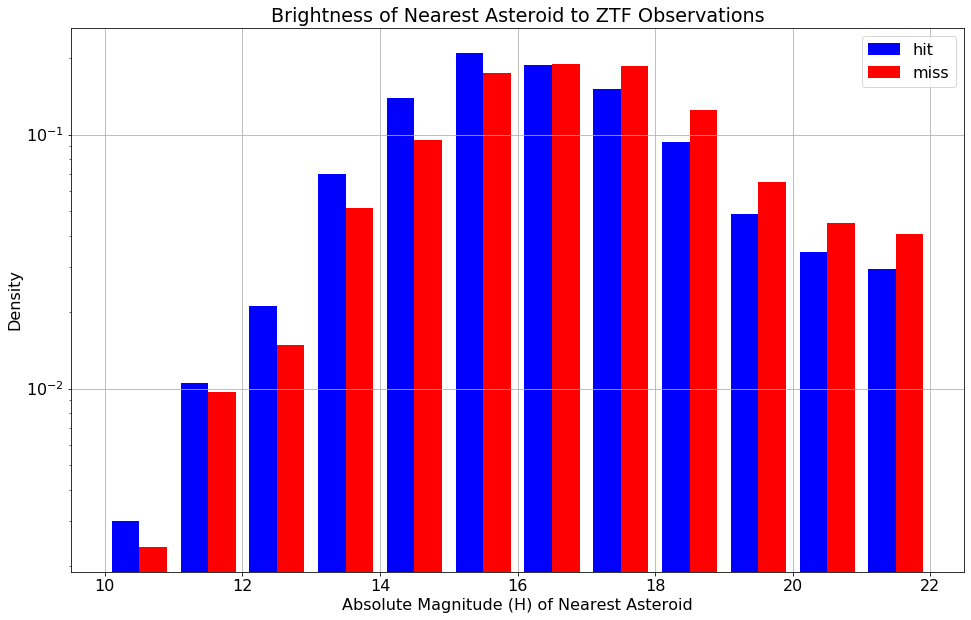
\includegraphics[width=1.0\textwidth]{../figs/ztf/nearest_ast_brightness.png}
\caption{Magnitude H of Nearest Asteroid to Each Detection\\
Hits are shown in blue, misses in red; a hit is a detection within 2.0 arc seconds of its expected direction.\\
The hits are slightly but noticeably tilted in favor of brighter asteroids.}
\end{center}
\end{figure}

I would like to take a step back and review what has been presented thus far.
Over 4 billion interactions between a ZTF asteroid detection and the predicted position of a known asteroid in the sky have been generated.
These have been filtered to associate each ZTF detection with the known asteroid it is nearest to.
This is a powerful enrichment of the original ZTF dataset, and might open the door to some additional work in the future.
For example, it could be used to create a bulk data set linking the original image files to the asteroids they belong to.
This could in turn be used to refine the machine learning pipeline used to classify detections and guess when they belong to the same object.

\section{Analyzing the Distribution of the Distance to the Nearest Asteroid}
\label{section_nearest_ast_distribution}
In this section I explore the statistical distribution of the Cartesian distance between observations and the nearest asteroid.
I compare the observed distribution of this distance to the theoretical distribution we would obtain 
if either our observed or predicted directions were distributed uniformly at random on the sphere.

\begin{figure}[hbt!]
\begin{center}
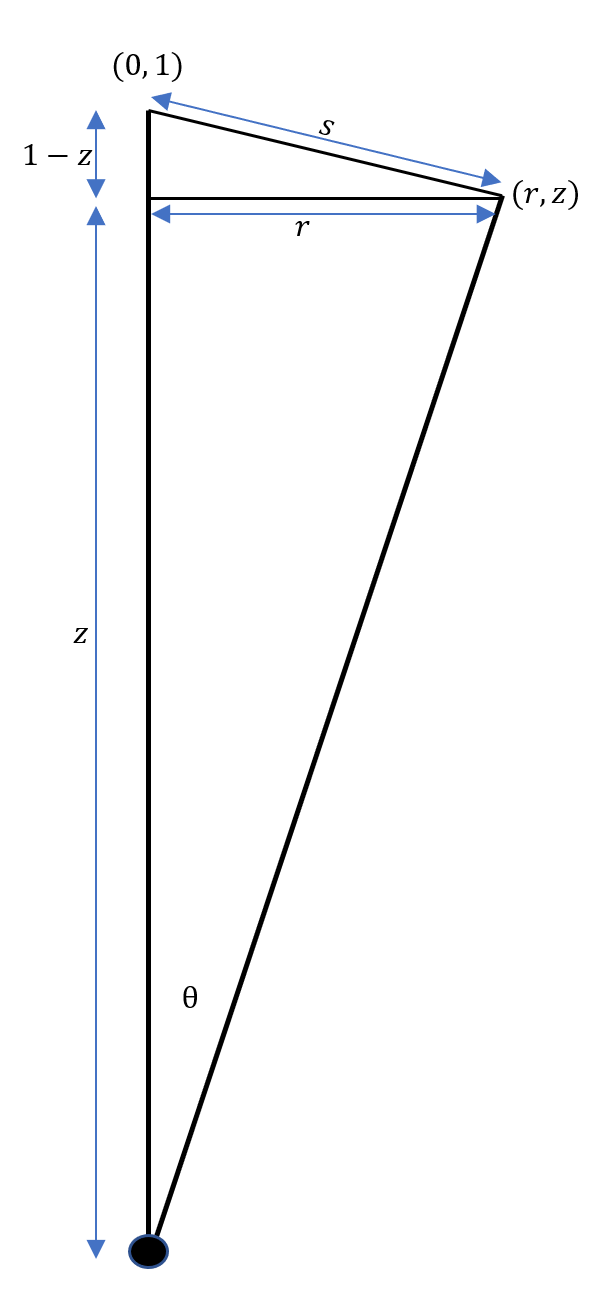
\includegraphics[width=0.36\textwidth]{../figs/misc/orange_slice.png}
\caption{Distance between an observation at the north pole and an arbitrary point.\\
The observed direction $\uobs$ is assumed w.l.o.g. to be at the north pole $(0, 0, 1)$.\\
The predicted direction $(x,y,z)$ is rotated in the $xy$ plane to to $(r, 0, z)$ \\
The Cartesian distance to from the observation to $(r,z)$ is $s$, the hypotenuse of a right triangle with sides $1-z$ and $r$.}
\end{center}
\end{figure}
Suppose without loss of generality that the observed direction is at the north pole, i.e. $\uobs = (0, 0, 1)$.
Suppose that the direction we predict is $(x, y, z)$.
Observe that the problem is symmetric about the $z$ axis, so we can rotate the problem into 
the plane containing the center, the north pole, and our guess.
Let $r^2 = x^2 + y^2$ be the squared distance from the $z$ axis to our guess.
This configuration is shown in the diagram above.
We can can relate the Cartesian distance $s$ to the height $z$ of our guess with the following simple observations.\\
$(x, y, z)$ lies on the surface of a sphere, so $x^2 + y^2 + z^2 = 1$.\\
$r^2 = x^2 + y^2$ by definition, so $r^2 = 1 - z^2$.\\
In our diagram, we can see that $s$ is the hypotenuse of a right triangle whose other two side have length $r$ and $1-z$.
Applying the Pythagorean Theorem, we find $s^2 = (1-z)^2 + r^s$. \\
This simplifies to
\begin{align*}
s^2 &= 2(1-z) \\
z &= 1 - \frac{s^2}{2}
\end{align*}
It turns out that this is a very useful parameterization because there is an elegant parameterization 
of the differential solid angle $d\Omega$ in terms of $dz$.
When surface integrals of a sphere are taught in introductory multivariate calculus courses, 
students are most likely to be exposed only to the surface element in spherical coordinates $(r, \theta, \phi)$ which is
$d\Omega = \sin \theta d\theta d\phi$.
See, e.g. \href{https://en.wikipedia.org/wiki/Spherical_coordinate_system}{Wikipedia - integration in spherical coordinates}.
But the parameterization in terms of the height $z$ along the $z$ axis is especially clean and convenient on this problem.\\
Observe that $z = \cos \theta$ so $dz = |- \sin \theta| d\theta = \sin \theta d\theta$.  
We take absolute values because this is an application of the change of variables formula and measures are always positive. \\
Substituting this expression for the surface element, we obtain
$$ d\Omega = dz \cdot d\phi$$
I call this result the ``orange slicing theorem.''
It tells you that if you slice an orange into horizontal slices, the amount of rind on each slice will be equal to $2 \pi$ times the height of the slice.

As a quick sanity check of this result, let's see if we can recover that the surface area of  the unit sphere is $4 \pi$:
$$ A = \int_{z = -1}^{1} \int_{\phi=0}^{2 \pi} d \phi dz = 2 \pi \int_{z = -1}^{1} dz = 4 \pi$$
We can now write the probability density function (PDF) for any function that can be expressed in terms of $z$.
Think of $Z$ as a random variable now.  The above result shows that when $Z$ is uniformly distributed on the unit sphere,
$$Z \sim \Unif(-1, 1)$$
Previously we showed that $z = 1 - s^2 / 2$.
This is a very useful result; it tells us that if we treat the squared distance as a random variable $S^2$, then it is uniformly distributed on $[0, 2]$.
Even more usefully, the conditional distribution of $S^2$, conditioned on $S^2 \le \tau^2$, is also uniform:
$$ S^2 | S^2 \le \tau^2 \sim \Unif(0, \tau^2)$$
If we apply a threshold distance $\tau$ and only consider predicted directions that are within Cartesian distance $\tau$ of an observation,
then the condtional distribution of the relative distance over the threshold squared is uniform on $[0, 1]$.
In mathematical notation instead of words, \\ 
Let $\upred$ be a random variable distributed uniformly on the unit sphere.\\
Let $S = \norm{\upred - \uobs}$ be the Cartesian distance between $\upred$ and $\uobs$. \\
Let $\tau$ be a threshold distance in [0, 2].\\
Let $V = S^2 / \tau^2$ be the relative squared distance of on observation vs. the threshold.\\
Then the conditional distribution of $V$, conditional on $S < \tau$ (equivalently $V < 1$) is
% $$V \sim \Unif(0, 1)$$

This describes the conditional distribution of distances we would see if we guessed one random direction in the sky.
But in this experiment, we are picking $733,489$ directions in the sky, one for each of the catalogued asteroids.
Then we are taking the minimum of these distances.
Can we still write down the conditional distribution of our nearest guess 
if they were indepedently and identically distributed (i.i.d.) at random as above?

Yes - Statistics 110 to the rescue!
Theorem 8.6.4: PDF of Order Statistics \cite{BH} states that if $X_1, \ldots X_n$ are i.i.d. continuous random variables
with PDF $f$ and CDF $F$, then the PDF of the $j$th order statistic (the $j$th smallest item $X_{(j)}$) is
$$f_{X_{j}})(x) = n \cdot {{n-1}\choose{j-1}} f(x) \cdot F(x)^{j-1} \cdot (1 - F(x))^{n-j}$$
In the special case that the $X_j$ are uniforms, this simplifies further (Example 8.6.5: Order statistics of Uniforms) \cite{BH}:\\
Let $U_1, \ldots U_n$ be i.i.d. $\Unif(0,1)$.
Then the distribution of $U_{j}$ is the Beta distribution,
$$U_{(j)} \sim \Beta(j, n-j+1)$$
The minimum is the order statistic of $j=1$, so
$$U_{(1)} \sim \Beta(1, n)$$ 

Let us now apply this theoretical result to compare our distribution of distances to what we would have obtained if 
we were randomly throwing darts into the sky so to speak.
The module \tty{ztf\_data\_viz} includes these calculations as well as the generation of charts.
\tty{cdf\_nearest\_dist} computes the theoretical CDF using the approach described above.
In the charts below, I will demonstrate that 2.0 arc seconds is a good threshold for classifying detections as ``hits'' against known asteroids.
For now, please treat it as a parameter I have chosen to demonstrate that these calculations work and are getting
astronomically more hits (no pun intended) than would arise from random chance.

Out of 5.69 million detections, 3.75 million (65.71\%) are within 2.0 arc seconds of the nearest catalogued asteroid.
The theoretical beta distribution says that if the predicted directions were distributed uniformly at random,
we would expect only 98 hits or 0.0017\% of the total be this close.
The immediate conclusion is that this whole set of calculations is working with a tolerance no worse than 2.0 arc seconds.

We can get a better intuition for what's happening by visualizing the histogram of distance to the nearest asteroid.
I initially plotted these against the percentile of the theoretical distribution; 
these plots would be a flat line with density 1 if the predicted directions were uniformly at random.
I found however that a simple plot of frequency vs. distance in arc seconds is easier to interpret 
once you've done the statistical analysis that the results are not due to chance.
Here is a plot showing hits inside a threshold of 2.0 arc seconds:
\begin{figure}[hbt!]
\begin{center}
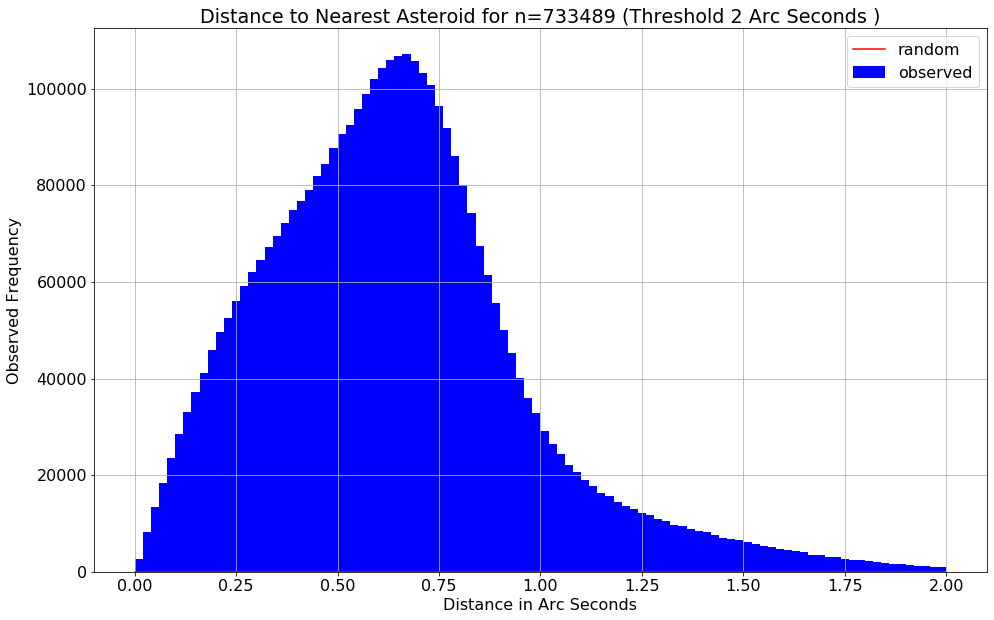
\includegraphics[width=1.0\textwidth]{../figs/ztf/nearest_ast_hist_dist.png}
\caption{Histogram of angular distance from each ZTF detection to the nearest asteroid in arc seconds.\\
These account for 65.57\% of the total data set.\\
The number of expected detections due to random chance is shown in red; it is visually indistinguishable from zero on the chart.}
\end{center}
\end{figure}

Here are two additional plot to visualize the distribution of distances between ZTF detections and the nearest known asteroid.
The first shows the absolute density in hits per square degree.
The second show the relative density of hits per square degree over what would have been expected
from the minimum of 733,489 guesses distributed uniformly at random on the sphere. \\
These charts seemed to have a shape that could be roughly approximated in a one parameter distribution as exponential.
They led me to propose a mixture model and log likelihood optimization objective function that I will describe in the next section
\begin{figure}[hbt!]
\begin{center}
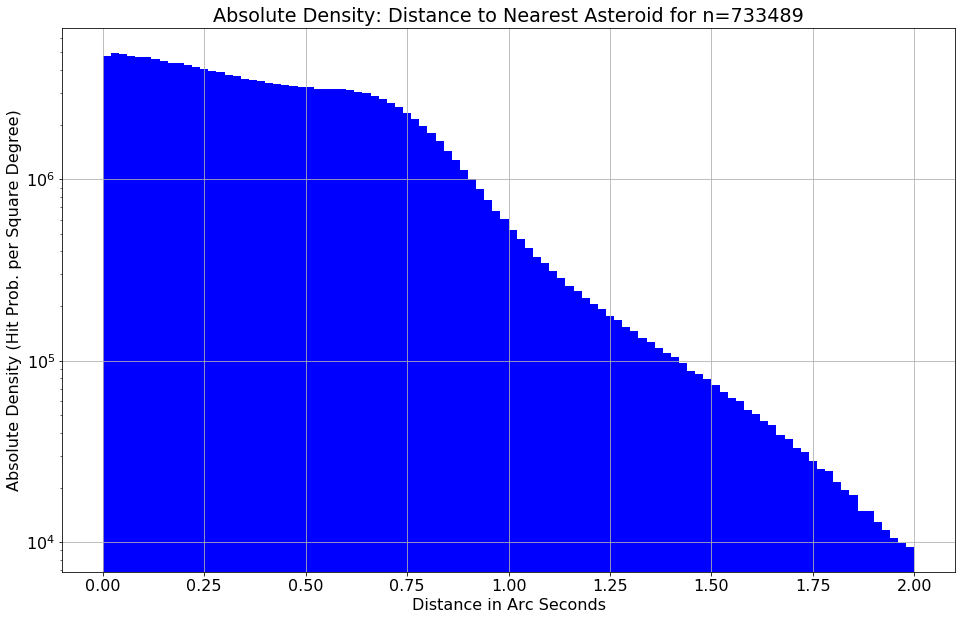
\includegraphics[width=1.0\textwidth]{../figs/ztf/nearest_ast_hist_dens_abs.png}
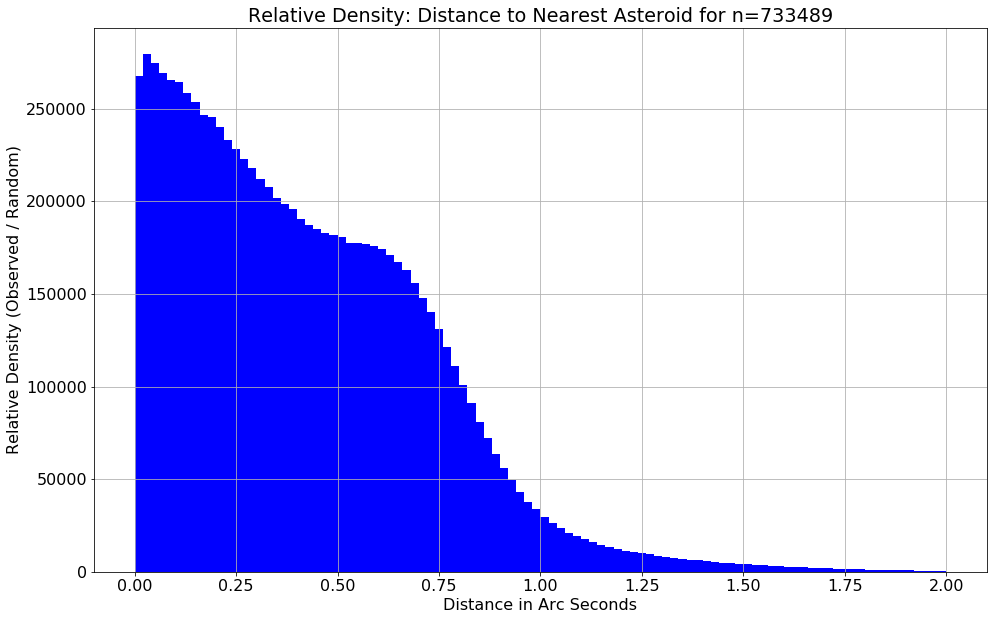
\includegraphics[width=1.0\textwidth]{../figs/ztf/nearest_ast_hist_dens_rel.png}
\caption{Density of hits for distance between ZTF detections and the nearest known asteroid. \\
The first chart shows the absolute density in hits per square degree.\\
The second chart shows the relative density of this over the baseline if the guesses were distributed randomly.}
\end{center}
\end{figure}
\clearpage

How many asteroids in the catalogue have enough detections in the ZTF dataset that we would have 
a sporting chance to recover their orbital elements from these observations alone?
Suppose for the sake of discussion that the number is $n=20$.
There are 63,746 asteroids with 20 or more hits at 2.0 arc seconds.
If we required only $n=10$ hits to recover the orbital elements, we could do it for 100,508 asteroids.\\
We can visualize this by plotting the cumulative frequency of close observations on the $y$ axis vs. hit count on the $x$ axis:
\begin{figure}[hbt!]
\begin{center}
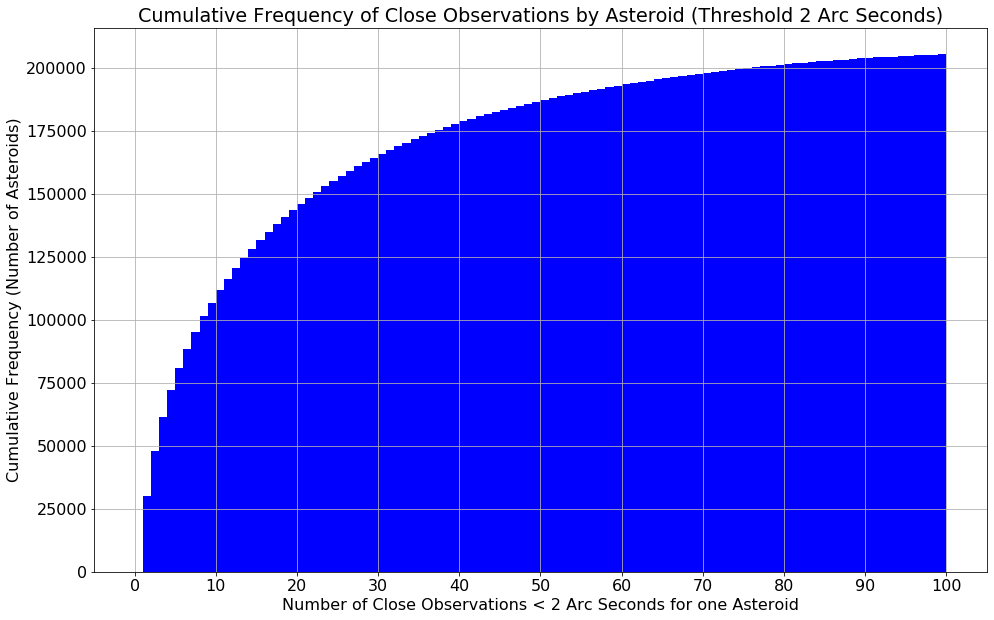
\includegraphics[width=1.0\textwidth]{../figs/ztf/nearest_ast_cum.png}
\caption{Cumulative frequency of asteroids by number of close observations < 2.0 arc seconds. \\
There are 63,746 asteroids with 20 or more close matches and 100,508 asteroids with 10 or more close matches. }
\end{center}
\end{figure}
\clearpage

\section{Conclusion}
\label{section_ztf_conclusion}
I have presented in this chapter an analysis of the asteroid detections in the ZTF astronomical data set.
I have demonstrated a calculation of the nearest known asteroid to each ZTF detection 
and the angular distance from that asteroid to the detection.
I have also developed the statistical distribution of distances that would be observed 
if the predicted directions were distributed uniformly at random on the sphere.
I have shown that of 5.7 million total ZTF detections, 65.7\% of them (almost two thirds)
are within 2.0 arc seconds of the predicted direction of the nearest known asteroid.
By comparing this number of hits to the number we would expect with a random baseline,
I have provided overwheliming evidence that this entire apparatus of data and calculations is accurate 
to a tolerance on the order of 2.0 arc seconds or better.
I have provided motivation that the approximate shape of the distribution of distances decays with an exponential tail.
Finally, I have shown the fraction of the asteroid catalogue we might be able to recover as a function of the number of observations required to fit it.  
If we require $n=10$ detections to verify or update the orbital elements of a known asteroid,
then we can apply this procedure on 100,508 asteroids representing 13.70\% of the known asteroid catalogue.